
\begin{figure*}
    \centering
    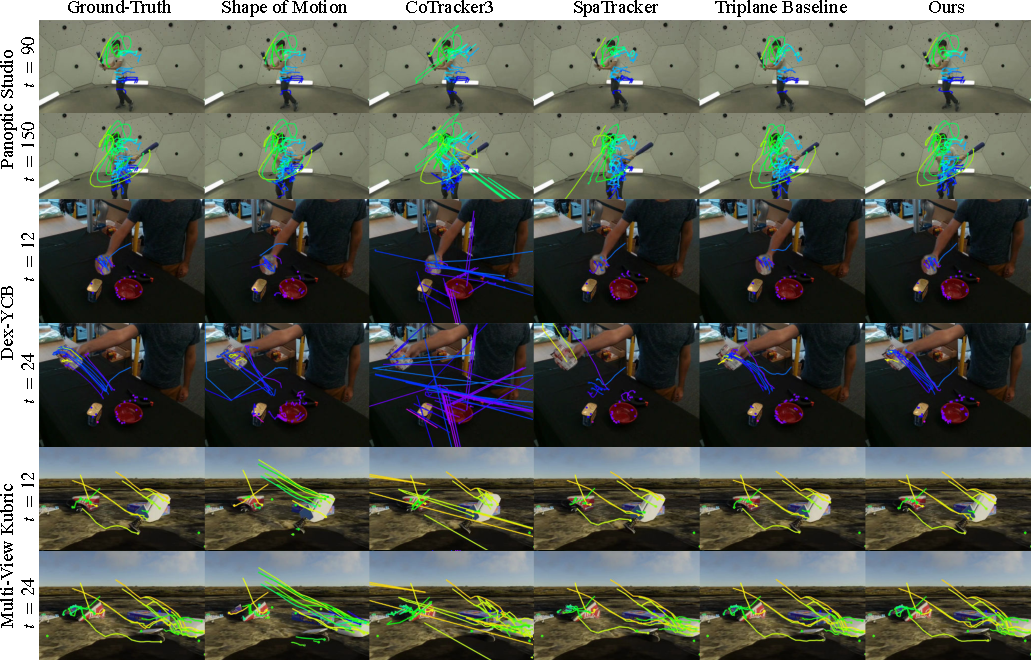
\includegraphics[width=\linewidth]{figures/qualitative_comparison.optimized-printer.pdf}
    \vspace{-0.25in}
    \caption{
    \textbf{Qualitative comparison of multi-view 3D point tracking.} We visualize results from a camera viewpoint \emph{not} used during inference (and not near the input cameras). Each pair of rows corresponds to two time steps from the same dataset. The leftmost column shows ground-truth 3D trajectories, while remaining columns depict predictions from different methods. Points predicted as occluded are indicated by empty circles. Compared to baselines, our method more accurately maintains correspondences across views and handles occlusions. Please see the supp. video and project page for additional visualizations. These examples correspond to the results in \cref{tab:main-results-table}.
    }
    \label{fig:qualitative}
    \vspace{-0.9cm}
\end{figure*}
